\documentclass[tikz,border=6pt]{standalone}
\usepackage{amsmath}
\usepackage{newtxtext,newtxmath}
\usetikzlibrary{arrows.meta,calc,decorations.pathreplacing}

\begin{document}
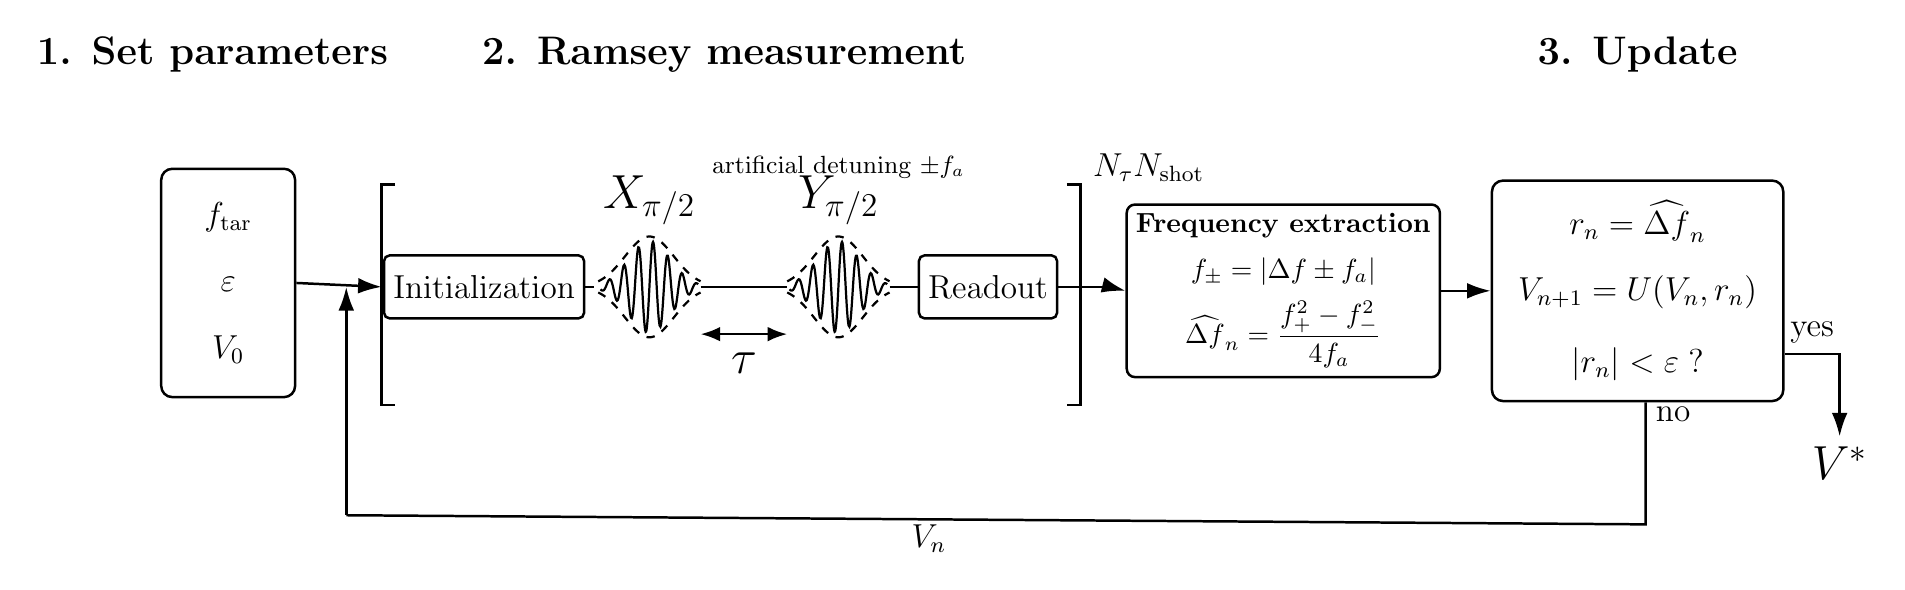
\begin{tikzpicture}[
  x=1cm,
  y=1cm,
  >=Latex,
  font=\large,
  line/.style={draw=black,line width=0.9pt},
  arrow/.style={line,-{Latex[length=3mm,width=2mm]}},
  block/.style={line,rounded corners=2pt,align=center,minimum height=0.8cm},
  setbox/.style={line,rounded corners=4pt,align=center,minimum width=1.7cm,minimum height=2.9cm},
  updatebox/.style={line,rounded corners=4pt,align=center,minimum width=3.7cm,minimum height=2.8cm},
  extractbox/.style={line,rounded corners=3pt,align=center,minimum width=3.25cm,minimum height=1.45cm,font=\normalsize},
  smallblock/.style={block,minimum width=1.6cm},
  pulse/.style={line,line width=0.8pt},
  envelope/.style={line,dashed,line width=0.8pt}
]

% Section headings
\node[font=\bfseries\Large] at (0.3,3.2) {1. Set parameters};
\node[font=\bfseries\Large] at (6.8,3.2) {2. Ramsey measurement};
\node[font=\bfseries\Large] at (18.4,3.2) {3. Update};

% Set parameters
\node[setbox] (set) at (0.5,0.3) {$f_{\mathrm{tar}}$\\[0.35cm]$\varepsilon$\\[0.35cm]$V_0$};

% Ramsey sequence bracket
\draw[line width=1pt]
  (2.62,1.55) -- (2.45,1.55) -- (2.45,-1.25) -- (2.62,-1.25);
\draw[line width=1pt]
  (11.15,1.55) -- (11.32,1.55) -- (11.32,-1.25) -- (11.15,-1.25);
\node[anchor=south west,font=\large] at (11.36,1.47) {$N_\tau N_{\mathrm{shot}}$};

% Ramsey blocks and signal line
\node[smallblock] (init) at (3.75,0.25) {Initialization};
\node[smallblock,minimum width=1.3cm] (readout) at (10.15,0.25) {Readout};
\draw[arrow] (set.east) -- (2.45,0.25);
\draw[line] (init.east) -- (5.15,0.25);
\draw[line] (8.95,0.25) -- (readout.west);
\draw[line] (readout.east) -- (11.70,0.25);

% Gaussian Ramsey pulses with dashed envelopes
\begin{scope}[shift={(5.85,0.25)}]
  \node[font=\LARGE] at (0,1.1) {$X_{\pi/2}$};
  \draw[pulse,domain=-0.62:0.62,samples=120,smooth]
    plot (\x,{0.58*exp(-7*\x*\x)*sin(deg(34*\x))});
  \draw[envelope,domain=-0.65:0.65,samples=80,smooth]
    plot (\x,{0.64*exp(-5.2*\x*\x)});
  \draw[envelope,domain=-0.65:0.65,samples=80,smooth]
    plot (\x,{-0.64*exp(-5.2*\x*\x)});
\end{scope}

\begin{scope}[shift={(8.25,0.25)}]
  \node[font=\LARGE] at (0,1.1) {$Y_{\pi/2}$};
  \node[font=\small] at (0,1.52) {artificial detuning $\pm f_a$};
  \draw[pulse,domain=-0.62:0.62,samples=120,smooth]
    plot (\x,{0.58*exp(-7*\x*\x)*sin(deg(34*\x))});
  \draw[envelope,domain=-0.65:0.65,samples=80,smooth]
    plot (\x,{0.64*exp(-5.2*\x*\x)});
  \draw[envelope,domain=-0.65:0.65,samples=80,smooth]
    plot (\x,{-0.64*exp(-5.2*\x*\x)});
\end{scope}

% Connecting lines around pulses
\draw[line] (6.50,0.25) -- (7.60,0.25);
\draw[line] (8.90,0.25) -- (8.95,0.25);

% Free evolution interval
\draw[Latex-Latex,line width=0.9pt] (6.50,-0.35) -- (7.60,-0.35);
\node[font=\LARGE] at (7.05,-0.72) {$\tau$};

% Update block
\node[extractbox] (extract) at (13.9,0.2)
  {\textbf{Frequency extraction}\\[0.16cm]
   $f_{\pm}=|\Delta f\pm f_a|$\\[0.16cm]
   $\widehat{\Delta f}_n=\dfrac{f_+^2-f_-^2}{4f_a}$};
\draw[arrow] (11.70,0.25) -- (extract.west);

\node[updatebox] (update) at (18.4,0.2)
  {$r_n=\widehat{\Delta f}_n$\\[0.35cm]
   $V_{n+1}=U(V_n,r_n)$\\[0.42cm]
   $|r_n|<\varepsilon\;?$};
\draw[arrow] (extract.east) -- (update.west);

% Output and decision paths
\draw[arrow] ($(update.east)+(0,-0.8)$) -- ++(0.7,0)
  node[midway,above] {yes} -- ++(0,-1.05)
  node[below,font=\LARGE] {$V^\ast$};

\draw[line] ($(update.south)+(0.1,0)$) -- ++(0,-1.55)
  node[right,pos=0.1] {no} -- (2.0,-2.65);
\draw[arrow] (2.0,-2.65) -- (2.0,0.25);
\node[font=\large] at (9.4,-2.95) {$V_n$};

\end{tikzpicture}
\end{document}
